\section{End Users}
\label{sec:enduser}
An end user is a person that will be using the final system.
Since we are using \scrum{} as our primary development practice we would prefer to have a product owner~\cite[p.~115]{Larman04} that can speak on behalf of the end users.
As mentioned in \secref{subsec:choosingmethod} we do not have one product owner thus will we facilitate the contact and communication with the end user group our self.
In this section we will define the group of end users for our \subsystem{} and shortly present the people that we use as representatives for this group -- we cannot speak with the entire group of potential end users, because it is simply too large.


\begin{figure}%
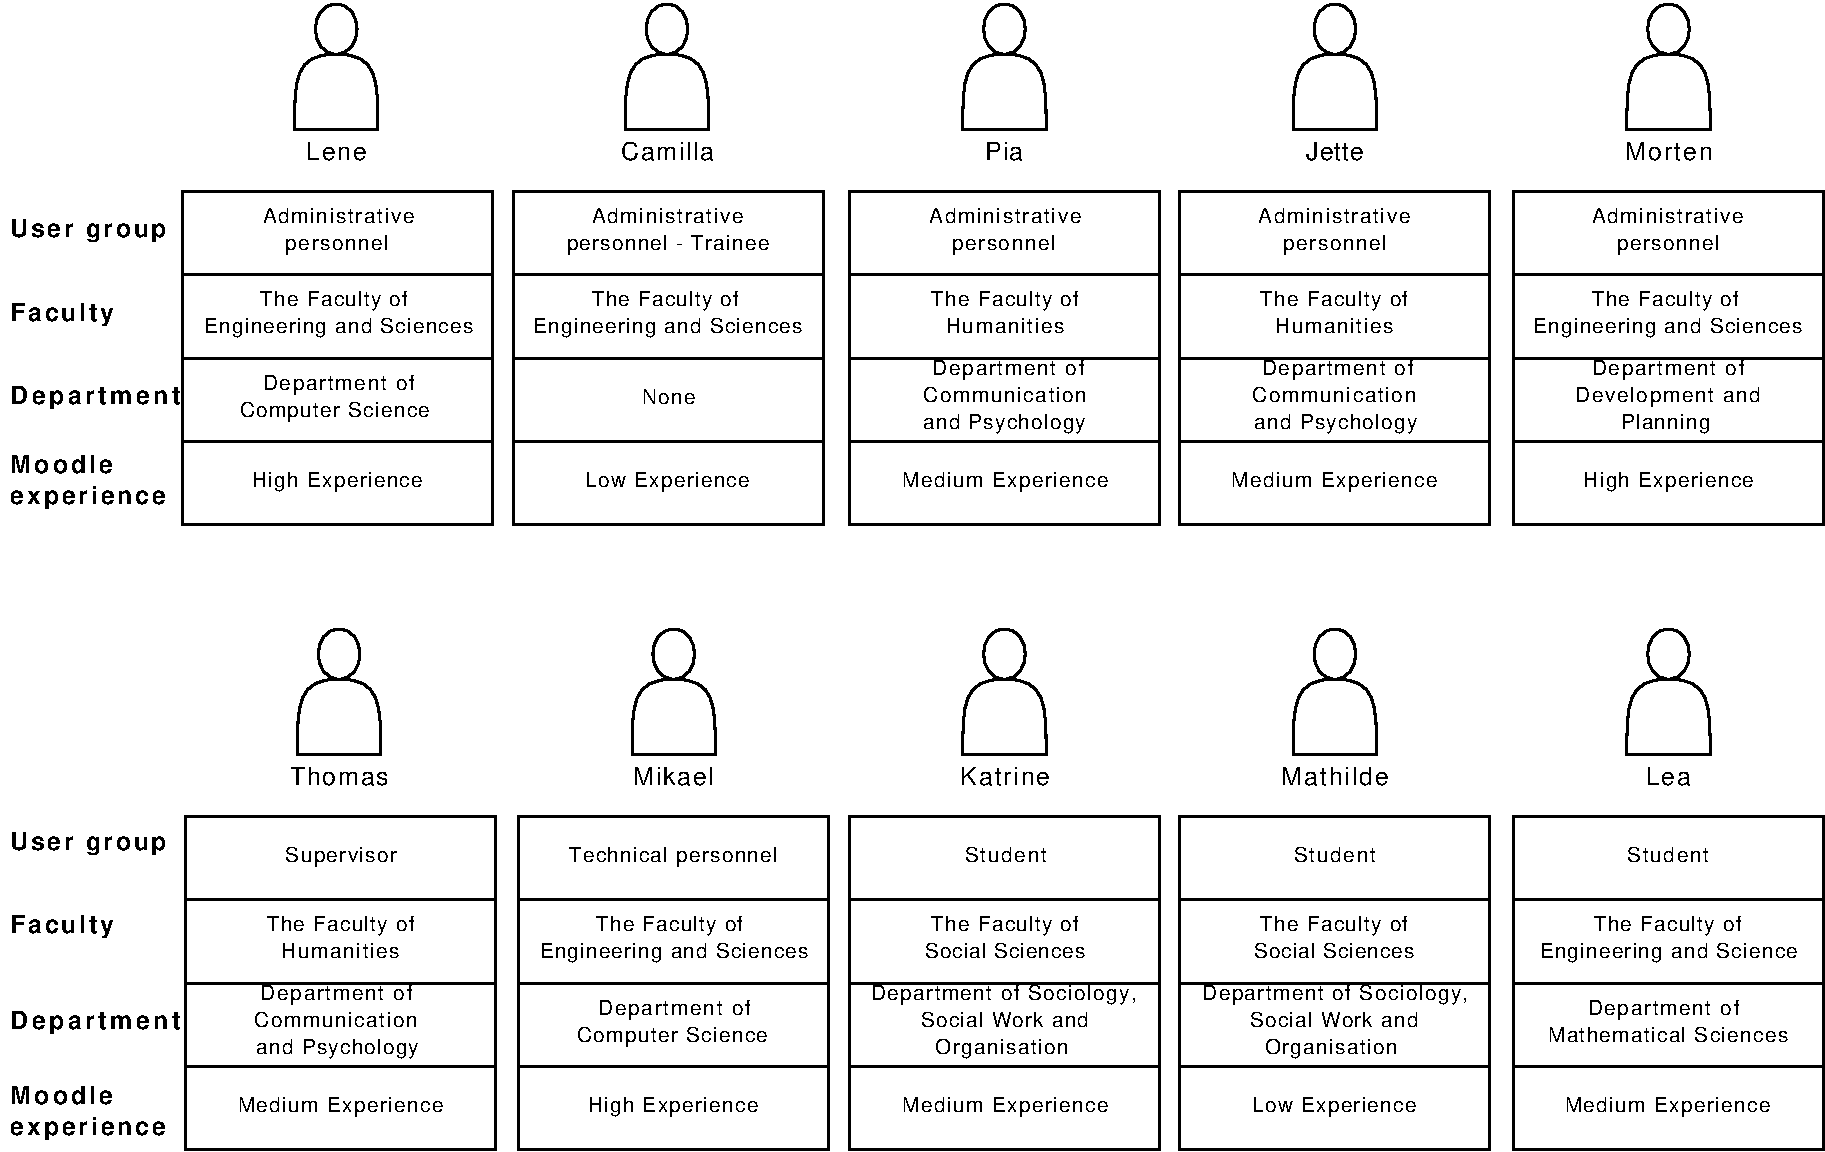
\includegraphics[width=\textwidth]{images/UserGroups}%
\caption{}%
\label{fig:usergroup}%
\end{figure}

\begin{comment}
For the full system the group of end users (also referred to as target group) is very diverse.
Roughly divided, it contains students, supervisors, and \admpers{} such as secretaries.
If we continue the division of students there are many dimensions to consider. 
For instance different students have different levels of experience with LMSs such as Moodle. Another dimension is that students have study at different faculties.
%The granularity may be even finer by partitioning by time of Moodle experience, such years of Moodle usage.
These different dimensions also apply to supervisors and \admpers{}.
We regard our target group as divided into two categories, users that are members of project groups and users that  manage project groups.
These categories may overlap.
In \secref{sub:endusersmembers} and \secref{sub:enduserstool} we present the characteristics of our target group.
%A table showing an overview of these two groups of end users is seen in \figref{fig:endusers}.
\end{comment}

For the full system the group of end users is very diverse.
In the \subsystem{} which we are developing we are interested in two different categories of end users.
\begin{itemize}
	\item The first group is the members of the project group.
	\item The second group is the managers of the virtual group room.
\end{itemize}
The user group that are members of the project group may very well be the same as the managers of the virtual group room. 
When choosing representatives for our user group there are several properties that we want cover.
In general we divide the user group into three types: \admpers{c}, supervisors, and students. 
In there different types we will focus on the following properties: Faculty and Moodle experience.
We would like to have representatives that cover these properties as much as possible.

In \secref{sub:endusersmembers} and \secref{sub:enduserstool} we will explore the two different categories of user groups.




%In \figref{fig:usergroup} a map of our different 



%Hvad har vi brug for at end users
%Hvad er deres properties

%Hvor og hvad har vi søgt efter da vi skulle finde target group 

%Hvad har vi fundet.




\subsection{Members of Project Groups}
\label{sub:endusersmembers}
As discussed in \chapref{chap:systemDef} our responsibility is to create the concept of a project group and creating a tool to manage these groups.
%For the concept of project group a group of students will function as our target group.
Since we are working together with three other peer-groups we will receive requests for functionality from them.
Our peer-groups have their own end users, both students and supervisors, where they get their requests from.
We can choose to regard students as a part of our end users and make our own field studies.
Alternatively we can choose to rely on our peer-groups requests and effectively use our peer-groups as our target group.
We choose a compromise and rely on our peer-groups requests and cooperate in the field studies related to the entire system or the concept of project groups.

The end users of project group functionalities are students and supervisors.
We want to have student representatives of different types, in particular students from different faculties.
We have two students from The Faculty of Social Sciences and one from The Faculty of Engineering and Sciences.
These are respectively Katrine Holmgaard Dinitzen, Mathilde Gammelgaard, and Lea Gustafsson.
Regarding supervisors, we choose to have a single representative; Thomas Ryberg Vibjerg Hansen~\cite{thomas}, who is supervisor under The Faculty of Humanities.
See \figref{fig:usergroup} for a review of our user group.
%We focus on students since our peer-group \supervisorgroup{}

\subsection{Users of Administrative Tool}
\label{sub:enduserstool}
Regarding the administrative tool, we choose to use administrative personnel as our main target group.
The end users we are using come from Aalborg University.
The reason for this is two-fold.
First reason is that we are implementing the Aalborg PBL model into Moodle, which means that Aalborg University come as a natural choice to look for end users.
Secondly our project is being conducted at Aalborg University, consequently it is easy for us to find personnel to participate.
To get a diverse group of end user we contact administrative personnel from our own institute and two other institutions at Aalborg University.
We also want our group of end user to contain both personnel well experienced in Moodle and other LMSs, and personnel inexperienced in Moodle.
From our own institute, Institute of Computer Science, we have the representatives Lene Winther Even~\cite{lene}, Camilla G\ae{}raa Larsen~\cite{camilla}, and Mikael M\o{}ller Hansen~\cite{mikael}.
Where the two former are a senior secretary and an office trainee respectively, and the latter an IT administrator
From The Faculty of Social Sciences we have been in contact with  Jette Due Nielsen~\cite{jette} and Pia Knudsen~\cite{piak} as our representatives.
We have also been in contact with Morten Mathiasen Andersen~\cite{morten} from MPBL in addition to the initial discussion discussed in \secref{sub:mpblInterview}.
See \figref{fig:usergroup} for a review of our user group.